\documentclass[12pt,a4paper]{article}

\usepackage{fontawesome5}
\providecommand{\faPencilAlt}{\faIcon{pencil-alt}}

\usepackage{styles/couleurs}
\usepackage{styles/mise_en_page}
\usepackage{styles/boites}
\usepackage{styles/maths}
\usepackage{styles/figures}

\usepackage{enumitem}
\usepackage{array}
\usepackage{tabularx}
\usepackage{amsmath}
\usepackage{amssymb}
\usepackage{tikz}
\usepackage{xparse}
\usepackage{pdflscape}
\usepackage{colortbl}

\usetikzlibrary{calc,arrows.meta,positioning}

\setlist[itemize]{leftmargin=1.4em,itemsep=0.15em,topsep=0.2em}
\setlist[enumerate]{leftmargin=*,itemsep=0.22em,topsep=0.25em}

\newcommand{\lignepointillee}{\noindent\dotfill\par\vspace{0.45em}}

\newcommand{\lignesreponse}[1]{%
\begin{tcolorbox}[
enhanced,colback=white,colframe=NeutreC!40,boxrule=0.5pt,arc=1.5mm,
left=3mm,right=3mm,top=2mm,bottom=1mm,before skip=2pt,after skip=2pt]
\foreach \i in {1,...,#1}{\lignepointillee}
\end{tcolorbox}}

\newcommand{\titreseq}[1]{%
\begin{center}
{\sffamily\LARGE\bfseries\color{TitreC}Séquence 7 -- Arithmétique}\\[0.2em]
{\sffamily\large\bfseries\color{SavoirC}#1}
\end{center}}

\newcommand{\grillecent}{%
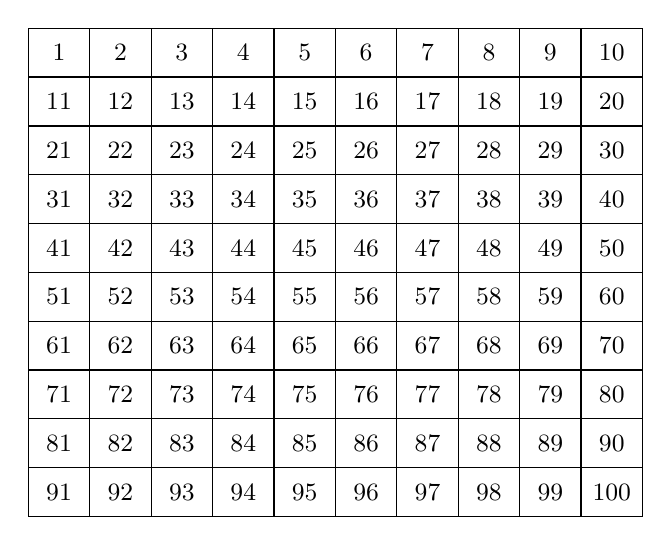
\begin{tikzpicture}[x=0.78cm,y=0.62cm]
  \foreach \n in {1,...,100}{
    \pgfmathtruncatemacro{\col}{mod(\n-1,10)}
    \pgfmathtruncatemacro{\lig}{9-floor((\n-1)/10)}
    \draw[line width=0.45pt] (\col,\lig) rectangle ++(1,1);
    \node[font=\small] at (\col+0.5,\lig+0.5) {\n};
  }
\end{tikzpicture}}

\begin{document}

\titreseq{Activité 5 -- Facteurs premiers et fractions égales}

\remarque{On utilise les facteurs premiers pour repérer les facteurs communs
au numérateur et au dénominateur.}

\section*{Partie A -- Une fraction à simplifier}

On considère la fraction :

\[
\frac{140}{135}.
\]

\begin{enumerate}
  \item Décompose \(140\) en produit de facteurs premiers.
  \item Décompose \(135\) en produit de facteurs premiers.
  \item Entoure les facteurs communs aux deux décompositions.
  \item Par quel nombre peut-on diviser le numérateur
        et le dénominateur ?
  \item Simplifie la fraction.
\end{enumerate}

\lignesreponse{7}

\section*{Partie B -- Écrire les étapes}

Complète.

\[
\frac{140}{135}
=
\frac{2\times2\times5\times7}
     {3\times3\times3\times5}
\]

\[
=
\frac{5\times(\ldots)}
     {5\times(\ldots)}
=
\frac{\ldots}{\ldots}.
\]

Pourquoi la valeur de la fraction ne change-t-elle pas ?

\lignesreponse{4}

\section*{Partie C -- Reconnaître des fractions égales}

Sans calculatrice, décompose les numérateurs et les dénominateurs
puis regroupe les fractions égales.

\[
\frac{14}{49}
\qquad
\frac{22}{55}
\qquad
\frac{34}{85}
\qquad
\frac{62}{155}
\]

\lignesreponse{8}

\section*{Partie D -- Simplifier}

Simplifie chaque fraction en utilisant les facteurs premiers.

\[
\frac{84}{126}
\qquad
\frac{105}{150}
\qquad
\frac{96}{168}
\qquad
\frac{165}{220}
\]

\lignesreponse{10}

\section*{Partie E -- Produire des fractions égales}

Complète avec deux fractions égales à \(\dfrac{6}{15}\) :

\[
\frac{6}{15}
=
\frac{\ldots}{\ldots}
=
\frac{\ldots}{\ldots}.
\]

Pour chaque égalité, indique si tu as multiplié ou divisé
le numérateur et le dénominateur par un même nombre.

\lignesreponse{4}

\aretenir{Pour produire une fraction égale, on multiplie ou on divise
le numérateur et le dénominateur par un même nombre non nul.

La décomposition en facteurs premiers permet de repérer tous les facteurs
communs utiles à la simplification.}

\end{document}
